\section{ARCHITECTURAL DESIGN}
\subsection{Overview} 
In this section is provided a complete overview of all the system components, from the logical level to the physical level of the PowerEnJoy service. First of all we give a description of the high level components and their interaction.\newline

\noindent From an high level prospective the service is composed by different modules allowing development and maintenance flexibility.This modularity allow also scalability for future service expansion, \todo{espandere il concetto} \newline

\noindent The main components of the system are:
\begin{itemize}
\item{\textbf{Database:}} the data layer of the service. All the persistent data will be stored in this layer.
\item{\textbf{Application Server:}} this component will manage the applicative logic.
\item{\textbf{Web Server:}} this layer is the interface with the world. It will manage the requests from the users and the website.
\item{\textbf{Mobile Application Interface:}} this is the interface between the Mobile User and the system. The user will use it to send requests to the web Server and see the results sent back through his mobile device. 
\item{\textbf{Car OnBoard Device:}} this is the module mounted on the car. It will communicate with the server and with the car ECU.
\item{\textbf{Web Site Interface:}} this is the interface between the Web User and the system.The user will use it to send requests to the web Server and see the results sent back through the web site. 
\end{itemize}

	\begin{figure}[H]	
	\centering
	\includegraphics[scale=0.5]{img/architecture_diagram}
	\caption{Architecture Diagram}
\end{figure}

All together, these components realize a 4-tiered architecture. In particular, the data layer, the presentation layer, the web server and the application server will have their own dedicated machine. The reasons why we made this choice concern:

\begin{itemize}
\item {\textbf{Security:}}
\item {\textbf{Scalability:}}
\item {\textbf{Performance:}}
\item {\textbf{Reliability:}}
\item {\textbf{Availability:}}
\end{itemize}

\todo{Bisogna scegliere se usare un'architettura a 3 o a 4 tier. 3--> web server e application logic insieme, 4--->separate}


\subsection{Component view} 
From a lower level perspective, the components of the system are:
\todo{Dubbio: Cosa va nel Web Server?}

\begin{itemize}
\item User Web Client GUI:
\item User Mobile Client GUI:
\item Driver Client GUI:
\item Data Manager:
\item Request Manager:
\item Account Manager:
\item Discount Manager:
\item Position Manager:
\item Travel Manager:

	\begin{figure}[H]	
	\centering
	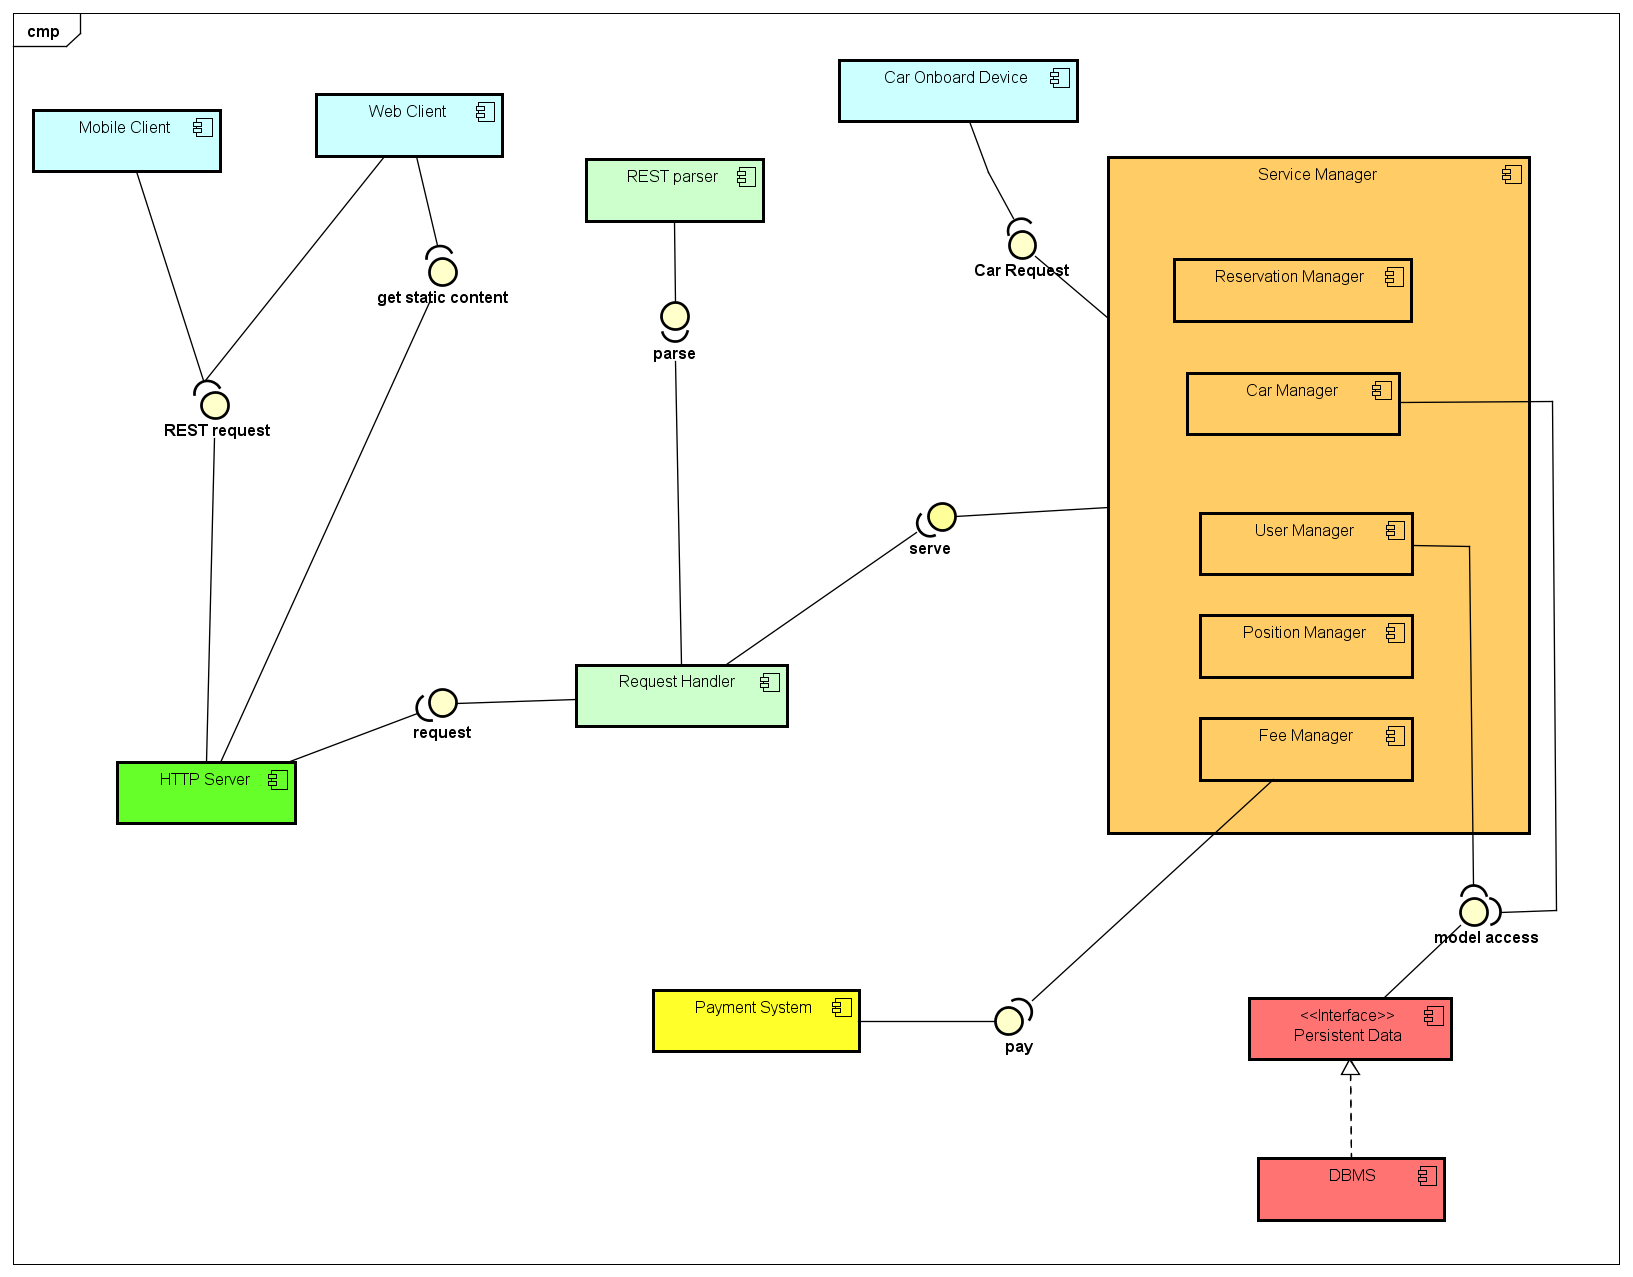
\includegraphics[scale=0.5]{img/Component_Diagram}
	\caption{Component Diagram}
	
	
\end{figure}

\end{itemize}


\subsection{Deployment view}
\subsection{Runtime view}
You can use sequence diagrams to describe the way components interact to accomplish specific tasks typically related to your use cases F. 
\subsection{Component interfaces} 
\subsection{Selected architectural styles and patterns}
Please explain which styles/ pattern you used, why, and how
\subsection{Other design decisions }